\section{Known Bugs and Problems}

This section contains an (incomplete) list of bugs and problems in \Voreen currently known to us.
Please feel free to contact us if any other problems arise while using \Voreen.

\subsection{No 2D Transfer Function Support}

Although the advanced transfer function editor includes an ``Intensity Gradient (2D)''-tab, 2D transfer functions
are currently not fully supported and may cause \Voreen to crash or show unexpected behavior.

\subsection{Color Map Interpolation in Animation Editor}

Generally the animation editor allows to animate the color map settings. However, using the default interpolation function to interpolate between the two different
color maps of two animation keys may not always yield the desired results. In some cases the interpolation might work (e.g. when 
using simple ramp transfer functions), in others it may cause rendering artefacts or unexpected color map states during playback. The boolean interpolation 
(which does not actually interpolate the color maps) may
be used to switch between the different color map settings set to the animation keys and should work without problems.

\subsection{Disappearing Quad View}

The \Voreen interface allows to drag the workspace description window and the properties window out of the default docked position and 
place it anywhere on the screen. 
However, this functionality may cause the quad view to disappear. An example of this behavior is depicted in figure \ref{fig:disappearing_quadview}. It seems
that this problem depends on the specific implementation of the Qt library. Unfortunately, the only solution is to restart \Voreen once the quad view has disappeared.

\begin{figure}[htb]
 \centering
 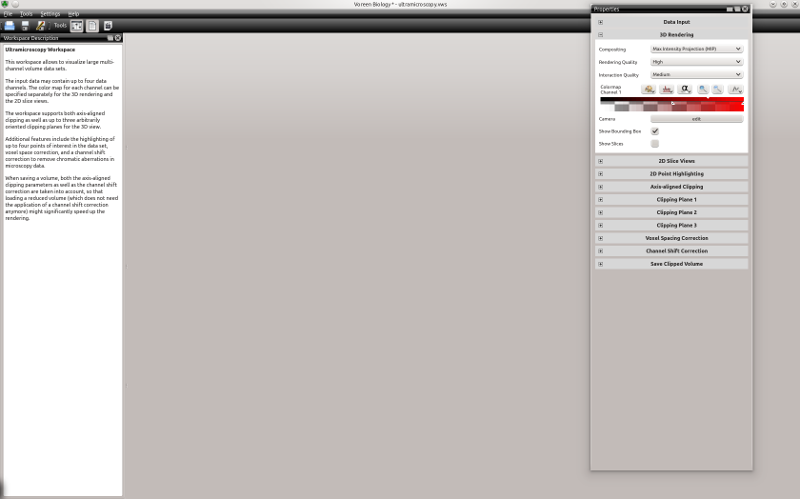
\includegraphics[scale=0.5,keepaspectratio=true]{./images/disappearing_quadview.png}
 % disappearing_quadview.png: 800x499 pixel, 90dpi, 22.58x14.08 cm, bb=0 0 640 399
 \caption{After dragging out the properties window, the quad view is not visible anymore.}
 \label{fig:disappearing_quadview}
\end{figure}


\subsection{TIFF Data Set Loading Problems}

If you encounter problems when loading TIFF-data sets, this may be based on missing header information in the image files. This is due to the fact that 
the TIFF format allows the header information for the data set to be stored either in each of the image files or only in the first file of the slice sequence.
When selecting a single file of the slice sequence, however, \Voreen will try to read the header information from the selected file, and, if the information 
is not present, report an error. To load your data set, you can either select the first file of the slice sequence in the loading dialogue, which should 
be including the header information, or configure the TIFF export in such a way that all of the single slice files include the header information.

\subsection{ATI/AMD-specific Problems}

Depending on the specific graphics card and driver version, several problems may occur when using \Voreen with AMD/ATI graphics cards.
This especially includes the \emph{channel shift correction} described in section \ref{ultramicroscopy.section.channelshift}, which might
crash on some AMD cards and drivers.